\section{Introduction}

Single-cell transcriptomics provides a high-resolution view of cellular heterogeneity, enabling the study of diverse cell states within complex tissues. However, these measurements are inherently sparse and noisy~\citep{luecken2019current}, making it difficult to reliably recover the underlying biological states. A common approach to address this challenge is to aggregate similar cells into \emph{metacells}, which provide denoised gene expression profiles that better reflect true cellular states. This relies on the assumption that variation within a group of similar cells is largely driven by noise, while shared patterns correspond to meaningful biological structure. Cell--cell affinity---a measure of pairwise similarity that guides which cells are grouped together---is central to this process and can in principle be derived from various biological sources.

Current metacell methods define this affinity based solely on gene expression and group cells that are close in this space. In multi-batch settings, however, batch effects distort gene expression, making similarity relationships reliable mainly within individual datasets. As a result, these metacell methods form aggregations within individual batches and fail to generalize across them, even though many biological states are shared. This limitation is particularly important for rare cell populations, where a single batch may not contain enough samples to recover stable cell states. In addition, existing methods rely primarily on transcriptomic similarity and ignore other sources of biological signal. In many settings, the spatial microenvironment~\citep{spatial1} influences cell state and can induce subtle but meaningful changes in gene expression. As a result, relying solely on transcriptomic similarity can miss consistent patterns driven by spatial organization, highlighting the need to consider multiple sources of similarity when grouping cells.

On the other hand, reconstruction-based models such as CVAEs can align cells across batches by learning shared representations, providing a strong signal for grouping cells with similar gene expression identity. However, because they optimize only for reconstruction, they do not explicitly preserve the local similarity structure defined by cell--cell affinities. As a result, they may distort biological information---for example, by merging rare but consistent patterns into larger groups, or overlooking subtle patterns defined by alternative similarity signals such as spatial context. 

These observations highlight a key limitation of existing approaches: methods that preserve similarity structure are typically restricted to predefined notions of similarity, while reconstruction-based methods align cells but do not preserve this structure. In practice, this leads to a trade-off between capturing meaningful cell--cell relationships and learning representations that are consistent across cells and datasets. Ideally, a model should leverage both sources of information---using reconstruction to capture valid gene expression patterns, while using affinity to guide which cells should be grouped together.

We introduce \textbf{scProto}, a framework that learns metacells by preserving affinity-defined relationships while remaining faithful to gene expression data (Figure~\ref{fig:overview}). Given one or more affinity graphs, scProto encodes cells into a latent space and learns a set of shared prototypes representing metacells. Cells are softly assigned to prototypes, and similarity between cells is defined through these assignments and aligned with the input affinity. This encourages highly connected cells to map to the same prototypes, preserving community structure of the affinity graph. At the same time, a reconstruction objective ensures that the learned representations capture meaningful gene expression patterns.

\begin{figure*}[t]
\centering
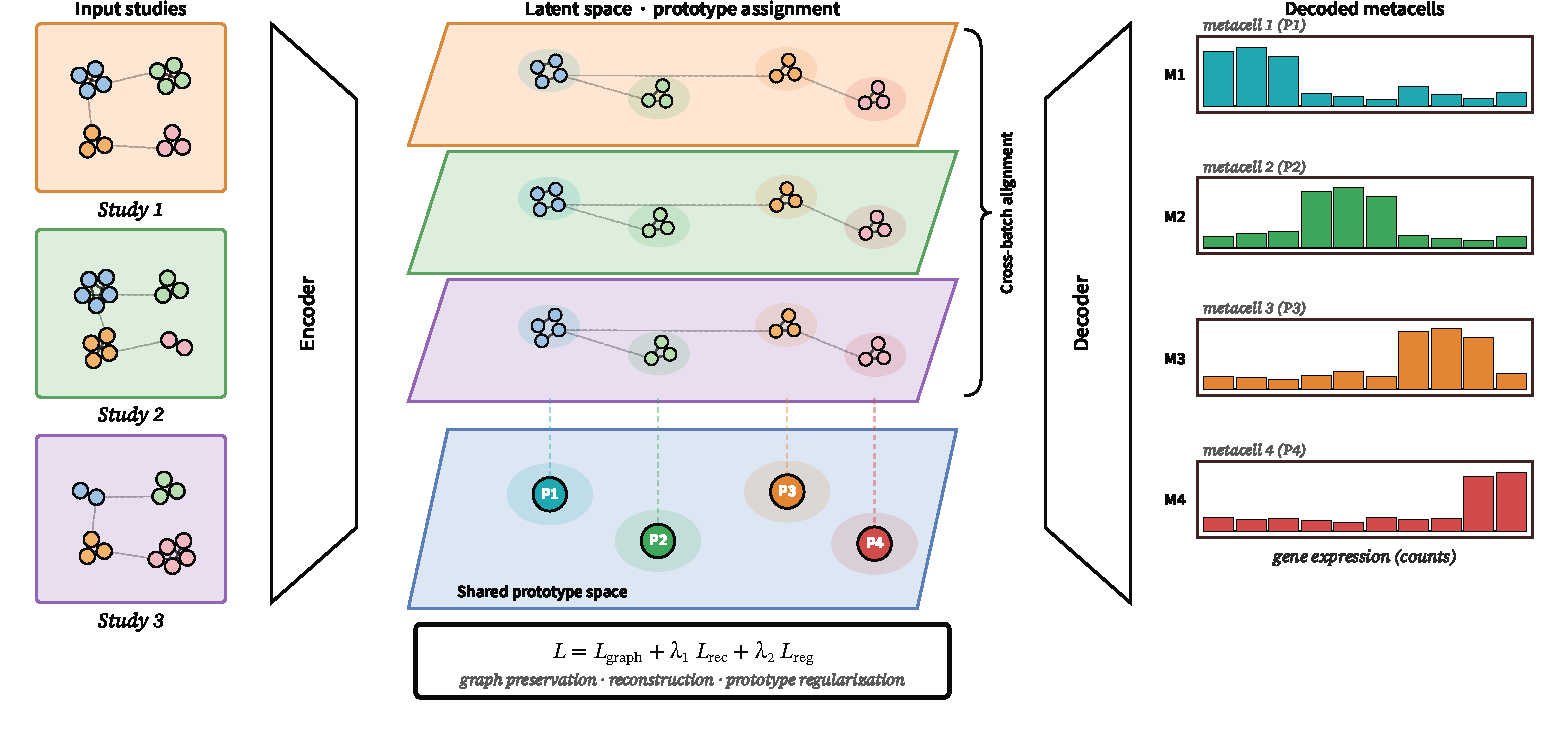
\includegraphics[width=\textwidth]{figures/scproto.pdf}
\caption{
Overview of scProto.
Given multiple datasets (batches), we construct similarity graphs and encode cells into a shared latent space.
Cells are softly assigned to a set of shared prototypes, which serve as metacells.
scProto preserves within-batch community structure via a community-preserving objective defined on prototype assignments,
while a reconstruction objective enables cross-batch alignment.
The learned prototypes represent shared, batch-invariant metacells decoded into gene expression space via a batch-conditional decoder.
}
\label{fig:overview}
\end{figure*}

We evaluate scProto on multiple single-cell and spatial transcriptomics datasets. Our results show that scProto forms metacells that integrate cells across batches while preserving within-batch structure, achieving high batch mixing without sacrificing modularity and cell-type purity. This leads to improved representation of rare cell populations, where cross-batch aggregation increases effective sample size and yields more stable metacells. The flexibility of the affinity framework extends naturally to spatial settings: by defining cell--cell affinity from spatial information, scProto captures microenvironmental structure more effectively than transcriptomics-only approaches, identifying metacells that reflect both cell identity and niche-specific variation.

Our contributions are as follows:
\begin{itemize}
    \item We introduce a prototype-based framework for learning cross-batch metacells that preserves affinity-defined community structure by modeling relationships through similarity in prototype assignments, rather than embedding distances, while maintaining fidelity to gene expression data.
    
    \item Our training objective combines a normalized association loss---which aligns prototype assignment patterns with affinity-defined community structure---and a coverage loss that prevents prototype collapse, enabling the model to learn compact and distinct metacell representations.
    
    \item We demonstrate that combining reconstruction with affinity guidance improves cross-batch aggregation, enhances representation of rare cell populations, and enables effective integration of spatial context.
\end{itemize}